\chapter{List coloring}

Firstly we can see a graph $G$ and its normal coloring which is depicted on a picture \ref{classic-coloring}. Whereas the list coloring shown on picture \ref{list-coloring} is that each vertex has a assigned list for which we can choose colors. Otherwise the coloring is the same.

\begin{figure}[!ht]
	\begin{subfigure}{0.45\textwidth}\centering
		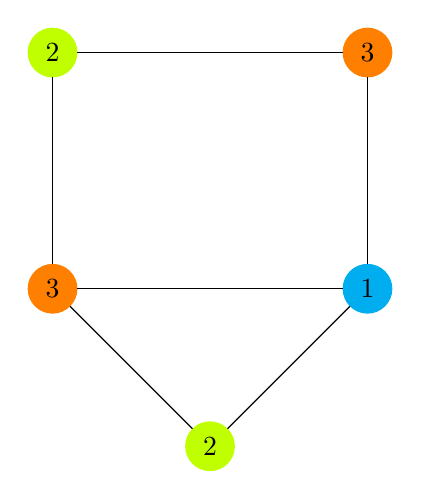
\begin{tikzpicture}[main/.style = {draw, circle, fill}]
			\node[main, color = lime] (1) at (0,0) {\textcolor{black}{2}};
			\node[main, color = orange] (2) at (-2,2) {\textcolor{black}{3}};
			\node[main, color = cyan] (3) at (2,2) {\textcolor{black}{1}};
			\node[main, color = lime] (4) at (-2,5) {\textcolor{black}{2}};
			\node[main, color = orange] (5) at (2,5) {\textcolor{black}{3}};
			\draw (1) -- (2);
			\draw (1) -- (3);
			\draw (2) -- (3);
			\draw (3) -- (5);
			\draw (2) -- (4);
			\draw (4) -- (5);
		\end{tikzpicture}
		\caption{Normal coloring of a graph $G$.}
		\label{classic-coloring}
	\end{subfigure}
	\begin{subfigure}{0.5\textwidth}\centering
		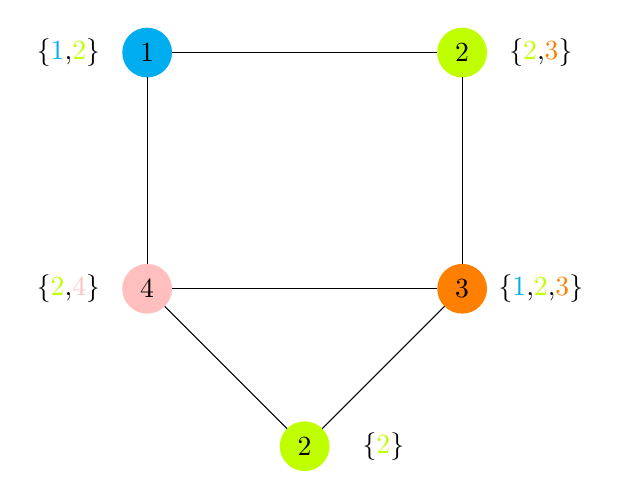
\begin{tikzpicture}[main/.style = {draw, circle, fill}]
			\node[main, color = lime] (1) at (0,0) {\textcolor{black}{2}};
			\node at (1,0) {\{\textcolor{lime}{2}\}};
			\node[main, color = pink] (2) at (-2,2) {\textcolor{black}{4}};
			\node at (3,2) {\{\textcolor{cyan}{1},\textcolor{lime}{2},\textcolor{orange}{3}\}};
			\node[main, color = orange] (3) at (2,2) {\textcolor{black}{3}};
			\node at (-3,2) {\{\textcolor{lime}{2},\textcolor{pink}{4}\}};
			\node[main, color = cyan] (4) at (-2,5) {\textcolor{black}{1}};
			\node at (3,5) {\{\textcolor{lime}{2},\textcolor{orange}{3}\}};
			\node[main, color = lime] (5) at (2,5) {\textcolor{black}{2}};
			\node at (-3,5) {\{\textcolor{cyan}{1},\textcolor{lime}{2}\}};
			\draw (1) -- (2);
			\draw (1) -- (3);
			\draw (2) -- (3);
			\draw (3) -- (5);
			\draw (2) -- (4);
			\draw (4) -- (5);
		\end{tikzpicture}
		\caption{List coloring of a graph $G$.}
		\label{list-coloring}
	\end{subfigure}
	\caption{Difference between basic and list coloring of a graph $G$.}
\end{figure}

\begin{defn}
	$k$-list-assignment is for an assignment for all vertices of size $k$.
\end{defn}

\begin{defn}
	The graph is $k$-list-colorable if $G$ can be colored by every $k$-list-assignment.
\end{defn}

\begin{defn}
	List chromatic number of a graph $G$ is denoted as $\chi_l(G)$. That is the min $k$ s.t. $G$ is $k$-list-colorable.
\end{defn}

\begin{observ}
	$\chi(G) \leq \chi_l(G)$
\end{observ}